\begin{figure*}[ht]
  \caption{System Architecture}
  \centering
    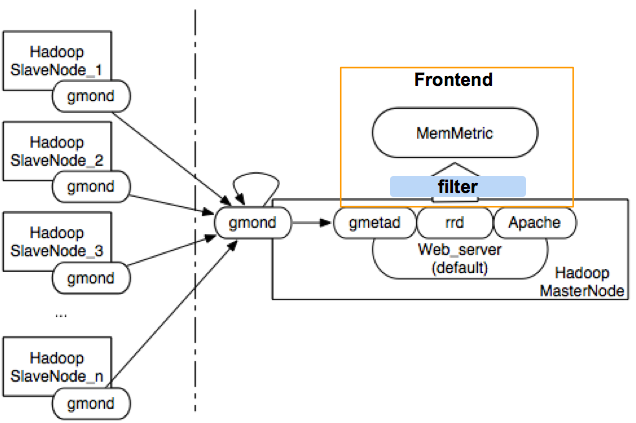
\includegraphics[width=4.0in]{image/architecture.png}
    \label{ref-architecture}
\end{figure*}

Figure \ref{ref-architecture} shows our system design. It contains three main components: \textbf{Metric gathering}, \textbf{Hadoop metric system}, and \textbf{Frontend}. We used Ganglia as the infrastructure to gather the  Hadoop cluster metrics in real-time. Hadoop cluster periodically reports its information to Ganglia daemon. After Ganglia collecting the metric information, they will be organized and visualized to users by our frontend system: Memmetric.

\subsection{Metric Gathering}

Ganglia deploys daemons on each node, called as gmond. Gmond in a worker node is responsible to collect monitoring statistics of a machine (e.g., CPU load, memory usage, disk load), and report those metrics to the gmond on the server node. 

Gmetad polls the metrics from the gmond on the server node, and stores the information into round robin database (rrd) periodically. 

Ganglia provides a web interface called ganglia-web, which can plots the metrics in rrds in the form of charts or json. 

We used ganglia-web as API server. Our frontend system queries ganglia-web for the information we needed, organize them, and visualize those information. 

\subsubsection{Ganglia Filter}

We found that Ganglia keeps to report finished task's metric as the last value it received. It makes the reported memory usage in a machine incredible large because the finished task memory usages are all counted into the sum of memory usage.

We added a filter inside the Ganglia API server to clean out the metrics of finished tasks. If one metric is continual reported as same value over tolerated period $T$, the filter will assume the task has finished, and remove the finished metric from reported API.

\subsection{Hadoop Metric System}

Hadoop 1.2.1 already provides metric system to gather different metrics source (e.g., Java Virtual Machine (JVM) metrics, Remote Procedure Call metrics) in Hadoop cluster and send them to the assigned destination (e.g., files or Ganglia daemon), shown in Figure \ref{figure-metric2}.

\begin{figure}[h!]
  \caption{Metric System in Hadoop (Metric2)}
  \centering
    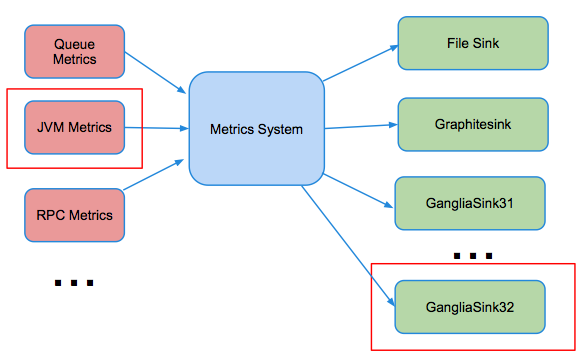
\includegraphics[width=0.5\textwidth]{image/ganglia32}
    \label{figure-metric2}
\end{figure}

In our system, we connected "JVM metrics" to metric system, and assigned them sending to Ganglia by GangliaSink. Therefore, Ganglia can receive task level memory usage information from Hadoop metric system.

We found that the default connector between metric system and Ganglia (GangliaSink31.java) behaves unexpectedly; therefore, we revised it to GangliaSink32 to monitor task level information, which is discussed in next section.

\subsubsection{Revised GangliaSink: GangliaSink32}

Each JVM in Hadoop cluster periodically reports it memory usage information into metric system as a key-value pair. The key format is jvm.metric.\{tag\}.heapMemoryUsedM. For example, jvm.metric.jvm\_20140405\_0001\_m\_1234.heapMemoryUsedM means the heap memory usage of the map task for Hadoop job 20140405\_0001. 

%[Figure?]

However, the original connector between metric system and Ganglia, GangliaSink31.java, will discard the tag of the reported metric key. For example, jvm.metric.jvm\_20140405\_0001\_m\_1234.heapMemoryUsedM will become jvm.metric.heapMemoryUsedM. 

\begin{figure}[h!]
  \caption{GangliaSink31 removes the tag in the key of metric and cause ambiguity.}
  \centering
    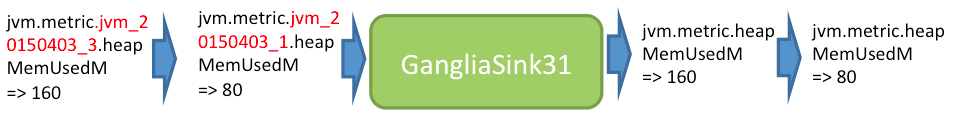
\includegraphics[width=0.5\textwidth]{image/ganglia31_flow.png}
\end{figure}

Removing the tag from the reported metric results in that the system cannot discriminate metrics from different running tasks. Therefore, the meaning of jvm.metric.heapMemoryUsedM becomes hard to explain, because we cannot know which target's memory usage does  jvm.metric.heapMemoryUsedM stands for. Also, the system cannot aggregate all task memory usage into a machine aspect memory usage, because they are all mixed in a metric. 

To solve this problem, we developed GangliaSink32.java to replace GangliaSink31.java. GangliaSink32.java can retain the tag of the metric key. Therefore, Ganglia can separate the memory usage information among different processes. 

\begin{figure}[h!]
  \caption{GangliaSink32 retains the tag in the key of metric.}
  \centering
    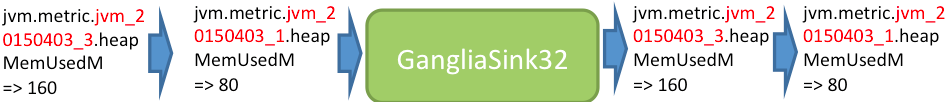
\includegraphics[width=0.5\textwidth]{image/ganglia32_flow.png}
\end{figure}

\subsection{Frontend: Memmetric}
We designed our frontend system (Memmetric) in two parts: \textbf{real-time monitor} and \textbf{historical monitor}. Real-time monitor  presents users the current status of the clusters. Historical monitor records anomalous data points to hint users debug their cluster.

\subsubsection{Real-time Monitor}

\begin{figure}[h!]
  \caption{Real-time Monitor}
  \centering
    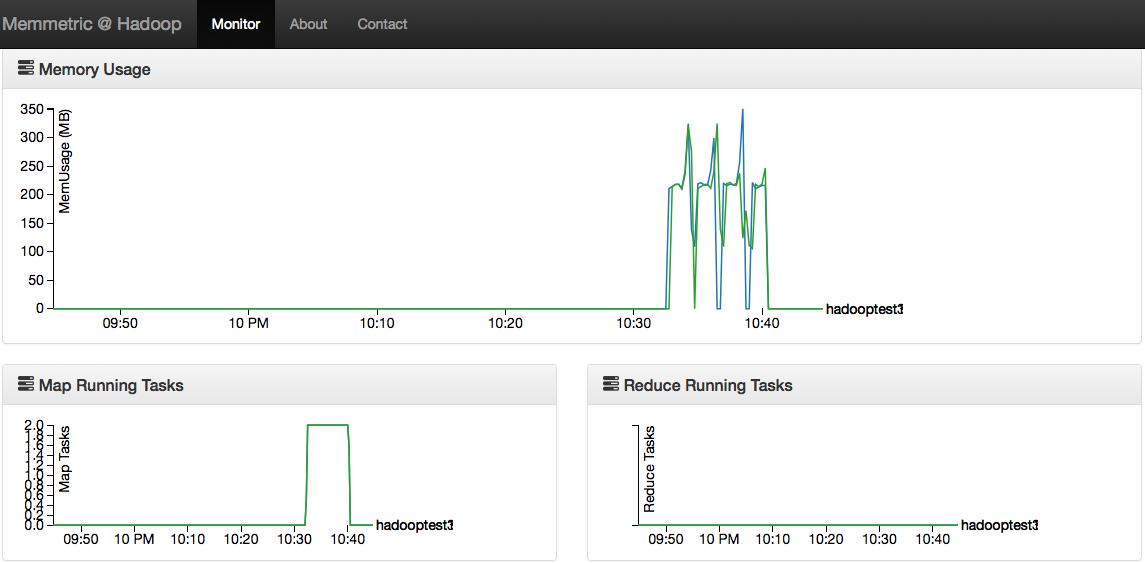
\includegraphics[width=0.5\textwidth]{image/real-time-monitor.png}
\end{figure}

Real-time monitor shows per-machine view of task heap memory usage, the number of running map tasks and reduce tasks. Each line in "Memory Usage" block shows the total heap memory usage in a machine. Also, lines in "Map Running Tasks" and "Reduce Running Tasks" show the number of map an reduce tasks in different machines.

Hadoop cluster reports the memory usage for each task to Ganglia. However, plotting the memory usage of all tasks individually on the same chart can be hard to understand, because a Hadoop job may spawn hundreds of tasks. Therefore, Memmetric aggregates all per-task heap memory usage (jvm.metrics.jvm\_\{process\_id and task type\}.memHeapUsedM) on a machine into a per-machine heap memory usage line. Also, Memmetric shows the number of running map tasks and reduce tasks. Real-time monitor provides a clue whether there are tasks killed due to over memory usage. If there is a sharp drop of heap memory usage on machine, it is possible that some tasks use too many memory to be killed by JVM or operating system. 

\subsubsection{Historical Monitor}

\begin{figure}[h!]
  \caption{Historical Monitor and Parameter Settings}
  \centering
    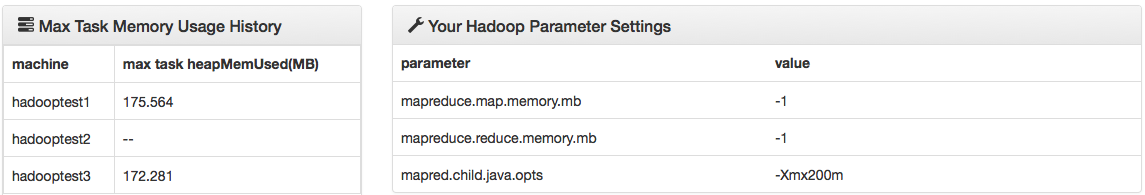
\includegraphics[width=0.5\textwidth]{image/historical-monitor.png}
\end{figure}

Historical monitor presents the odd data points in each machine for users to revise their cluster parameter settings. Memmetric records the data points of largest task heap memory usage in each machine, because those points are the possible moments where a task violates the memory upper bound restriction and results in failure. For example, if Hadoop cluster sets "mapred.child.java.opt" as "-Xmx200m", which means that  the JVM child of a task at most allocate 200MB memory. If the historical monitor shows that some task has used more than 200MB, it is highly possible that the task will be killed, and the user should consider to modify the parameter to enlarge the maximum heap memory usage.

Besides, Memmetric crawls the configure files in Hadoop directory (i.e. "hadoop/conf") to fetch the parameter settings, and shows them nearby historical monitor. Users can revise their cluster's settings by comparing historical monitor and parameter settings. 

\begin{figure}[h!]
  \caption{Memmetric Overview}
  \centering
    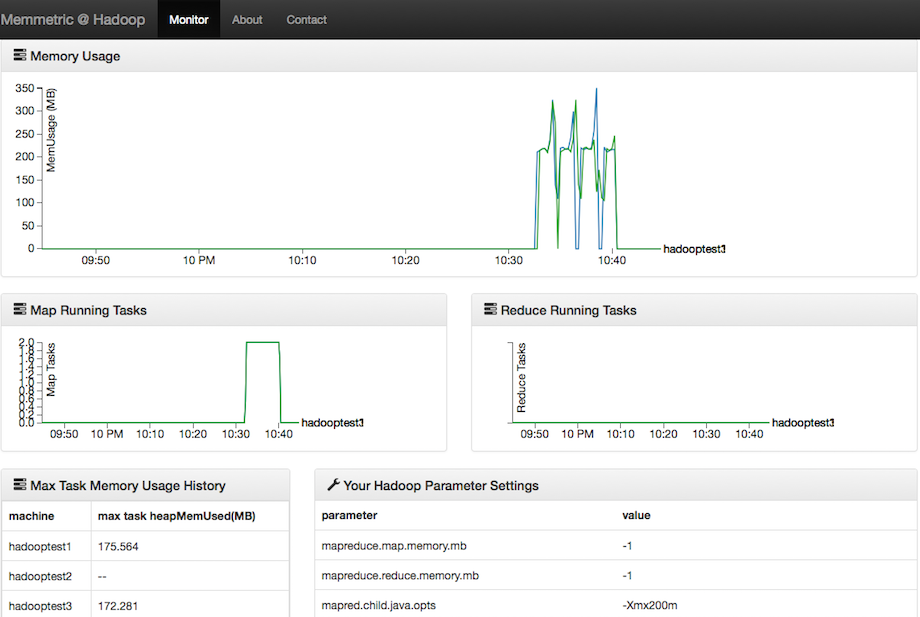
\includegraphics[width=0.5\textwidth]{image/overview.png}
\end{figure}

